% Exemplo 2 da cinemática inversa: pose calculada no plano do braço (cm)
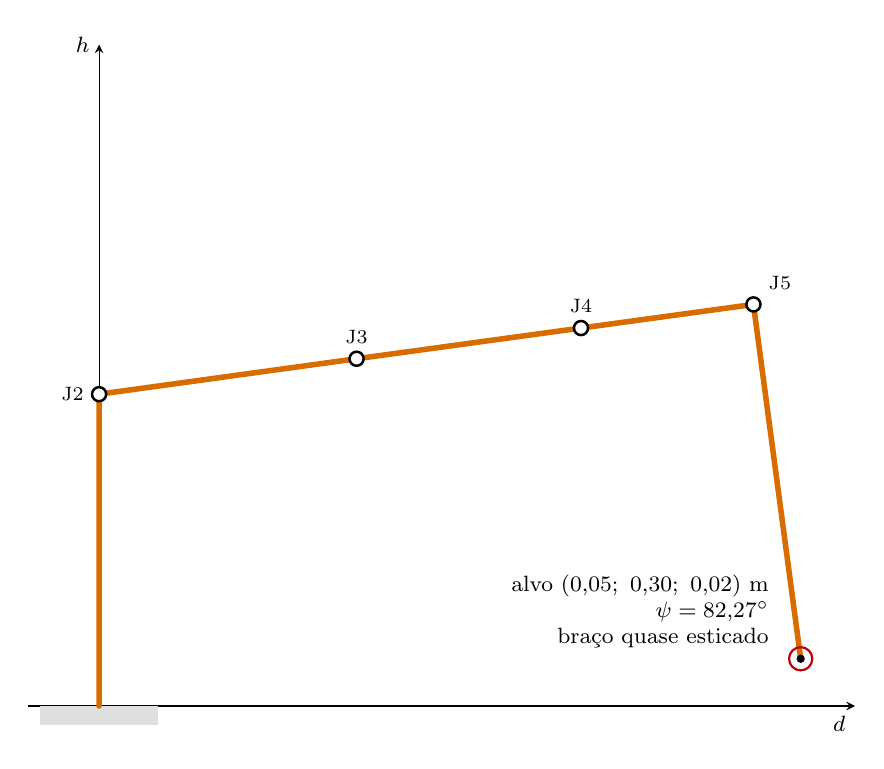
\begin{tikzpicture}[scale=0.3, >=stealth,
    elo/.style={line width=2pt, line cap=round},
    junta/.style={circle, draw, fill=white, line width=0.9pt, inner sep=1.8pt},
    every node/.style={font=\footnotesize}]
  \draw[->, thin] (-3,0) -- (32,0) node[below left] {$d$};
  \draw[->, thin] (0,0) -- (0,28) node[left] {$h$};
  \fill[gray!25] (-2.5,-0.8) rectangle (2.5,0.0);
  \draw[elo, orange!85!black] (0.0,0.0) -- (0.0,13.2) -- (10.9,14.7) -- (20.4,16.0) -- (27.7,17.0) -- (29.7,2.0);
  \foreach \p/\n/\a in {(0.0,13.2)/J2/left, (10.9,14.7)/J3/above, (20.4,16.0)/J4/above, (27.7,17.0)/J5/above right}
    { \node[junta] at \p {}; \node[\a=2pt, font=\scriptsize] at \p {\n}; }
  \fill (29.7,2.0) circle (5pt);
  \draw[red!75!black, thick] (29.7,2.0) circle (14pt);
  \node[left=8pt, align=right] at (29.7,4.0) {alvo $(0{,}05;\ 0{,}30;\ 0{,}02)$ m\\$\psi = 82{,}27^\circ$\\braço quase esticado};
\end{tikzpicture}